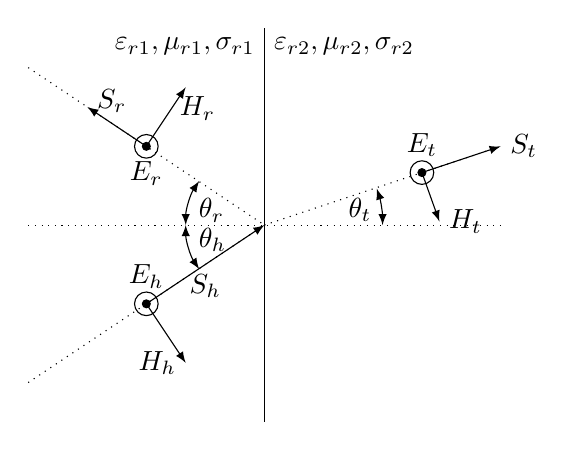
\begin{tikzpicture}
    \tikzset{cross/.style={cross out, draw=black, minimum size=2*(#1-\pgflinewidth), inner sep=0pt, outer sep=0pt},
        %     %default radius will be 1pt. 
        cross/.default={3.5pt}}
    %Kreuz
    \draw[dotted] (-3,0) -- (3,0);
    \draw[-] (0,-2.5) -- (0,2.5)                
        node[below right]   {$\varepsilon_{r2}, \mu_{r2}, \sigma_{r2}$}
        node[below left]    {$\varepsilon_{r1}, \mu_{r1}, \sigma_{r1}$};
    %Rücklaufende
    \draw[-latex] (-1.5,1) -- (-2.25,1.5)   node[right, yshift=.5ex]{$S_r$};
    \draw[-latex] (-1.5,1) -- (-1,1.75)     node[below, xshift=1ex] {$H_r$};
    \draw[-] (-1.5,1) circle (0.15)         node[below,yshift=-.5ex]{$E_r$};
    \draw[-,fill=black!100] (-1.5,1) circle (0.05);
    \draw[dotted] (-3,2) -- (0,0);
    \draw[latex-latex] (146:1) arc (146:180:1) 
        node[midway, right, yshift=-.7ex] {$\theta_r$};

    %Hinlaufende
    \draw[-latex] (-1.5,-1) -- (0,0)        node[below, midway]         {$S_h$};
    \draw[-latex] (-1.5,-1) -- (-1,-1.75)   node[left]                  {$H_h$};
    \draw[-] (-1.5,-1) circle (0.15)        node[above, yshift=.5ex]    {$E_h$};
    \draw[-,fill=black!100] (-1.5,-1) circle (0.05);
    \draw[dotted] (-3,-2) -- (0,0);
    \draw[latex-latex] (180:1) arc (180:214:1)
        node[midway, right, yshift=.7ex] {$\theta_h$};

    %Transmitierte
    \draw[-latex] (2,0.6666) -- (3,1)           node[right] {$S_t$};
    \draw[-latex] (2,0.6666) -- (2.2223,0.0448) node[right] {$H_t$};
    \draw[-] (2,0.6666) circle (0.15)           node[above, yshift=.5ex] {$E_t$};
    \draw[-,fill=black!100] (2,0.6666) circle (0.05);
    \draw[dotted] (0,0) -- (3,1);
    \draw[latex-latex] (0:1.5) arc (0:18:1.5)
        node[midway, left, yshift=-.3ex] {$\theta_t$};

\end{tikzpicture}